\documentclass{beamer}

\usetheme{Frankfurt}
\beamertemplatenavigationsymbolsempty
\setbeamertemplate{footline}[frame number]

\usepackage[ngerman]{babel}
\usepackage[babel]{csquotes}
\usepackage[utf8]{inputenc}
\usepackage{listings}
\usepackage{color}
\definecolor{darkgray}{rgb}{0.4, 0.4, 0.4}
\definecolor{purple}{rgb}{0.65, 0.12, 0.82}
\definecolor{darkgreen}{cmyk}{0.7, 0, 1, 0.5}

\lstset{
  language=Python,
  basicstyle=\ttfamily,
  keywordstyle=\color{blue}\bfseries,
  ndkeywordstyle=\color{darkgray}\bfseries,
  identifierstyle=\color{black},
  commentstyle=\color{purple}\ttfamily,
  stringstyle=\color{red}\ttfamily,
  showspaces=false,
  showstringspaces=false,
  showtabs=false,
  framesep=2mm,
  tabsize=4,
  captionpos=b,
  breaklines=true,
  breakatwhitespace=true,
  numberbychapter=false,
  aboveskip=0.25cm,
  belowskip=0.25cm,
  inputencoding=utf8
}

\usepackage{graphicx}
\usepackage{hyperref}
\usepackage{verbatim}

\urlstyle{same}
\hypersetup{pdfpagemode=FullScreen,pdfpagelayout=SinglePage,pdfstartview=Fit}

\date{19.12.2012}
\subject{Webapplikationen mit Flask}
\title{Webapplikationen mit Flask}
\author{Adrian Mönnich}
\institute[Hochschule Karlsruhe]{
  Fakultät für Informatik und Wirtschaftsinformatik\\
  Hochschule Karlsruhe
}



\begin{document}
\maketitle
\section*{Überblick}
\frame{\tableofcontents}


\section{Motivation}
\begin{frame}
  \frametitle{Motivation}
  
\includegraphics[width=0.6\textwidth]{images/python-logo.png} \hspace*{\fill}
  \newline
  \hspace*{\fill} 
\includegraphics[width=0.5\textwidth]{images/flask-logo.pdf}
\end{frame}


\section{Python}
\begin{frame}[fragile]
  \frametitle{Python}
  \begin{itemize}
    \item Dynamische Programmiersprache
    \item Oftmals als Skriptsprache genutzt
    \item Mehrere Paradigmen
    \item Blöcke werden durch Einrückung definiert
  \end{itemize}

  \begin{exampleblock}{Python-Code}<2>
    \begin{lstlisting}
def hello_world():
    if False:
        print 'World demise on 2012-12-21.'
    print 'Hello World.'
    \end{lstlisting}
  \end{exampleblock}
\end{frame}

\begin{frame}[fragile]
  \frametitle{WSGI}
  \begin{itemize}
    \item Web Server Gateway Interface
    \item Python-Standard PEP-333: \url{http://www.python.org/dev/peps/pep-0333}
    \item Schnittstelle zwischen Webservern und Python-Applikationen
    \item WSGI-Applikationen sind \emph{callables} (also z.B. Funktionen)
  \end{itemize}
  \begin{exampleblock}{Hello WSGI}<2>
    \begin{lstlisting}
def application(environ, start_response):
    start_response('200 OK', [('content-type', 'text/plain')])
    return ['Hello World!']
    \end{lstlisting}
  \end{exampleblock}
\end{frame}

\section{Flask}
\begin{frame}
  \frametitle{Allgemeines}
  \begin{itemize}
    \item Microframework für Webapplikationen
    \item Sehr komfortabel zu nutzen - \enquote{Flask is Fun}
    \item Ausführliche Dokumentation
    \item \enquote{based on Werkzeug, Jinja 2 and good intentions}
    \item Open Source (BSD-Lizenz)
  \end{itemize}

  \begin{block}{BSD-Lizenz}<2>
    \begin{itemize}
      \item Kopieren, Verändern, Weitergeben ist erlaubt
      \item Copyright-Vermerk des Originals darf nicht entfernt werden
      \item Änderungen können unter einer beliebigen Lizenz veröffentlich werden (auch proprietär)
    \end{itemize}
  \end{block}
\end{frame}

\begin{frame}
  \frametitle{Aufbau}
  \begin{itemize}
    \item Application: Zentrale Klasse und WSGI-Anwendung (implementiert \lstinline{__call__()})
    \item Blueprints: Module, die eigene Routen, Templates, etc. enthalten können. Erlaubt bessere
          Strukturierung einer komplexeren Anwendung
    \item Routing: Mapping von URLs auf Python-Funktionen
    \item Sessions: Signierte Cookies
    \item Templates (Jinja 2)
    \item Signals: Hooks um z.B. vor jedem Request Code auszuführen
  \end{itemize}
\end{frame}

\begin{comment}
\begin{frame}
  \frametitle{Werkzeug}
  \begin{itemize}
    \item \enquote{WSGI utility library}
    \item Debugger
    \item Request/Response-Klassen
    \item Hilfsfunktionen für HTTP (Cookies, Dateiuploads, \ldots)
    \item URL-Routing
    \item \url{http://werkzeug.pocoo.org}
  \end{itemize}
\end{frame}
\end{comment}

\section{Flask-Tutorial}

\begin{frame}
  \frametitle{Zielsetzung}
  \begin{itemize}
    \item Ein einfaches Feedback-Formular zu Flask selbst
    \item Zufrieden/unzufrieden inkl. kurzer Begründung
    \item Real existierende Applikation: \url{http://feedback.flask.pocoo.org}
    \item Quellcode: \url{https://github.com/mitsuhiko/flask-feedback}
  \end{itemize}

  \begin{exampleblock}{Screenshot}
    \begin{center}
      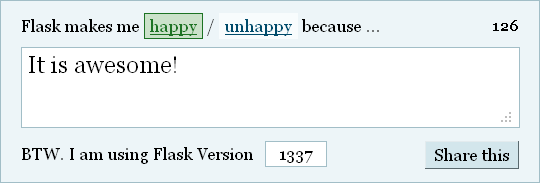
\includegraphics[width=0.5\textwidth]{images/flask-feedback.png}
    \end{center}
  \end{exampleblock}
\end{frame}

\begin{frame}
  \frametitle{Wieso ein Feedbackformular?}
  \begin{itemize}
    \item Einfache Applikation
    \item Datenbankanbindung
    \item Formularverarbeitung
    \item Nur wenige Python-Packages bzw. Flask-Extensions benötigt
    \item Verwendet mit Flask-SQLAlchemy die wichtigste Flask-Erweiterung
  \end{itemize}
\end{frame}

\begin{frame}
  \frametitle{Einschub: Flask-Extensions}
  \begin{itemize}
    \item Erinnerung: Flask ist ein Microframework
    \item Zusätzliche Funktionalität durch Erweiterungen
    \item Flask-SQLAlchemy: Einbindung des Datenbankframeworks \emph{SQLAlchemy}
    \item Flask-Script: Kommandozeilenbefehle
    \begin{itemize}
      \item Dev-Server inkl. Debugger
      \item Python-Shell
      \item Benutzerdefinierte Befehle (oftmals \emph{createdb} und \emph{dropdb})
    \end{itemize}
  \end{itemize}
\end{frame}

\begin{frame}[fragile]
  \frametitle{Initialisierung}
  \begin{itemize}
    \item Flask initialisieren
    \item Defaultwerte für die Konfiguration
    \item Konfigurationsdatei laden
    \item Flask-SQLAlchemy initialisieren
  \end{itemize}
  \begin{exampleblock}{Eine Flask-Anwendung wird geboren\ldots}
    \begin{lstlisting}
app = Flask(__name__)
app.config['FEEDBACK_PER_PAGE'] = 30
app.config.from_pyfile('settings.cfg')
db = SQLAlchemy(app)
    \end{lstlisting}
  \end{exampleblock}
\end{frame}

\begin{frame}
  \frametitle{Einschub: Flask-SQLAlchemy}
  \begin{itemize}
    \item Initialisierung der SQLAlchemy-Session
    \item Fassade für diversen häufig benötigte SQLAlchemy-Objekte
    \item \lstinline{db.Model} ist die Basisklasse für alle Mappings
    \item Basiert auf \lstinline{declarative_base()} von SQLAlchemy
    \item Enthält zusätzliche Erweiterungen
      \begin{itemize}
        \item \lstinline{Feedback.query.filter(id=42).all()}
        \item \lstinline{Feedback.query.paginate()}
      \end{itemize}
  \end{itemize}
\end{frame}

\begin{comment}
\begin{frame}[fragile]
  \frametitle{Datenbankmodell}
  \begin{itemize}
    \item Nutzung des in SQLAlchemy enthaltenen ORMs
    \item Nur eine einzige Tabelle benötigt
    \item Tabellenname wird implizit aus dem Klassennamen gebildet
  \end{itemize}
  \begin{exampleblock}{Definition des SQLAlchemy-Modells}
    \begin{lstlisting}
class Feedback(db.Model):
    id = db.Column(db.Integer, primary_key=True)
    kind = db.Column(db.Integer)
    text = db.Column(db.String(1000))
    version = db.Column(db.String(40))
    pub_date = db.Column(db.DateTime)
    \end{lstlisting}
  \end{exampleblock}
\end{frame}
\end{comment}

\begin{frame}[fragile]
  \frametitle{Routing}
  \begin{exampleblock}{Routen in der Feedback-Anwendung}
    \begin{lstlisting}
@app.route('/', methods=('GET', 'POST'))
def give_fb():
    pass

@app.route('/message/<int:id>')
def show(id):
    pass

@app.route('/happy', defaults={'page': 1})
@app.route('/happy/page/<int:page>')
def happy(page):
    pass
    \end{lstlisting}
  \end{exampleblock}
\end{frame}

\begin{frame}[fragile]
  \frametitle{Anwendungslogik}
  \begin{exampleblock}{View-Funktion der \enquote{Give Feedback}-Seite}
    \begin{lstlisting}
def give_fb():
    if request.method == 'POST':
        text = request.form['feedback']
        if len(text) <= 140:
            fb = Feedback(text=text)
            db.session.add(fb)
            db.session.commit()
            return redirect(
                url_for('show', id=fb.id))
        return redirect(url_for('give_fb'))
    return render_template('give_fb.html')
    \end{lstlisting}
  \end{exampleblock}
\end{frame}

\begin{comment}
\begin{frame}
  \frametitle{Einschub: Jinja 2}
  \begin{itemize}
    \item Standard-Templateengine von Flask
    \item Auch separat verfügbar
    \item Kompiliert Templates zu Python-Bytecode
    \item Template-Vererbung
    \item Optionale Sandbox
    \item Autoescaping (HTML)
    \item \url{http://jinja.pocoo.org}
  \end{itemize}
\end{frame}
\end{comment}

\begin{frame}[fragile]
  \frametitle{Jinja2-Template}
  \begin{exampleblock}{Template der \enquote{Give Feedback}-Seite}
    \begin{lstlisting}[syntax=HTML]

Give Feedback

 <h2>We Love Feedback</h2>
 <form action="{{request.url}}" method=post>
  <p class=text>
   <textarea name=feedback cols=50 rows=2>
   </textarea>
 </form>

    \end{lstlisting}
  \end{exampleblock}
\end{frame}

\section{Fazit}
\begin{frame}
  \frametitle{Fazit}
  \begin{itemize}
    \item Komfortables Webframework
    \item Kein Bloat
    \item Rapid Application Development
    \item Browserbasierter Debugger
    \item Gut lesbarer Code (übersichtlich und sinnvoll kommentiert)
    \item Doku und ausführliches Tutorial auf \url{http://flask.pocoo.org}
  \end{itemize}
\end{frame}

\end{document}
